\documentclass{article}
\usepackage[utf8]{inputenc}

\usepackage{graphicx}
\usepackage{float}
\usepackage{subcaption}
\usepackage{changepage}
\usepackage[ruled,vlined]{algorithm2e}
\usepackage{url}

\usepackage{geometry}
\geometry{margin=1.7in}
\usepackage[nottoc,numbib]{tocbibind}
\usepackage[export]{adjustbox}[2011/08/13]

\usepackage[labelfont=bf]{caption}

\begin{document}

\title{Optimizing TV Content for Video on Demand, Leveraging Image Retrieval for Unsupervised Detection of Recurring Content in TV Shows\'{} Video Files}
\author{Master Thesis\\ \\ Niels ten Boom  \\ s4767314}

\date{\vspace{-3ex}}

\maketitle
\newpage

\tableofcontents
\newpage

\section{Introduction} \label{introduction}
Viewing rates for TV are dropping gradually while the user counts of streaming services such as Netflix and Videoland are growing year over year. This shift from TV to Video on Demand introduces new problems for broadcasters, as they now have to support a hybrid form of traditional broadcasting and Video On Demand (VOD). In this thesis we consider a method to help improve the user experience for VOD.

Video content is optimized for just one form, and currently that is TV. This means that the video content contains recurring content consisting of: recaps, opening credits, bumpers (to ease a viewer into commercials), closing credits and previews. A viewer watching this content back-to-back may find it preferable to be able to skip this recurring content to improve their viewing experience. Providing this functionality to users, requires metadata on where the skippable content occurs in the videos. For a large percentage of their content, such metadata has not been retained. Videoland currently hosts over 1000 different titles consisting of multiple seasons and episodes and this selection is always changing. An automated solution that can detect this content in videos would be very useful to transform the video content into a format suited for VOD. In this thesis we will explore the best methods for such an automated solution.
% Definities van series?

There is little margin for error with this solution. The accuracy of the end result should be sufficiently high enough for it to be trusted to label all of the content automatically. If that is not the case then it needs double checking by a human. Because if a part of the video gets mislabeled, a user may skip over actual content. It is critical to RTL that this does not happen.

This thesis presents research on unsupervised detection of recaps, opening credits, bumpers, closing credits and previews given the video files from a TV-show. We are going to attempt to tackle this problem by using image retrieval techniques. The motivation behind this is that the general characteristic of the segments is that they reoccur. To be able to detect recurring content we are going to compare similarities of frames across content, this should be done efficiently and accurately, both attributes are important in image retrieval research. Our main research question then is:
\newline
\begin{adjustwidth}{0.3in}{0.3in}
\textit{\textbf{How well do image retrieval methods perform in accurately detecting recurring content across a TV-show?\newline}}
\end{adjustwidth}
With the subquestions: \\
\begin{adjustwidth}{0.3in}{0.3in}
	\textit{\textbf{How can image retrieval be used to detect recurring content?\newline}}\\
	\textit{\textbf{How accurate is each image retrieval approach?\newline}}\\
	\textit{\textbf{How can the best method be utilized in practice?\newline}}
\end{adjustwidth}
This thesis aims to answer aforementioned research questions. The rest of this section will be used to expand on the different type of video classes which this research is focused on. Section \ref{relatedwork} explains all of the related work. In section \ref{section:imageretrieval} image retrieval and the used methods are expanded upon. Section \ref{methodology} describes the data and methodology and then the produced results are presented in section \ref{results}. Lastly, the results are discussed in section \ref{discussion}.

\subsection{Recurring Content Classes} \label{section:segmentclasses}
In this section we will give a background on the different types of content to be detected. What all the content classes have in common is that they (partially) reappear in previous or future episodes. We will use this attribute for the detection. 

\subsubsection{Closing Credits}
The closing credits at the end of a video contain a lot of scrolling text most of the time and there is little variation between the frames. In these texts everybody related to the production of the video is mentioned. In general the frames all have a black background with white text. But backgrounds can also vary as can be seen in figure \ref{closingcredits}, therefore a solution that simply detects black and white would not suffice.

\begin{figure}[H]
  \centering
  \begin{subfigure}[b]{0.4\textwidth}
    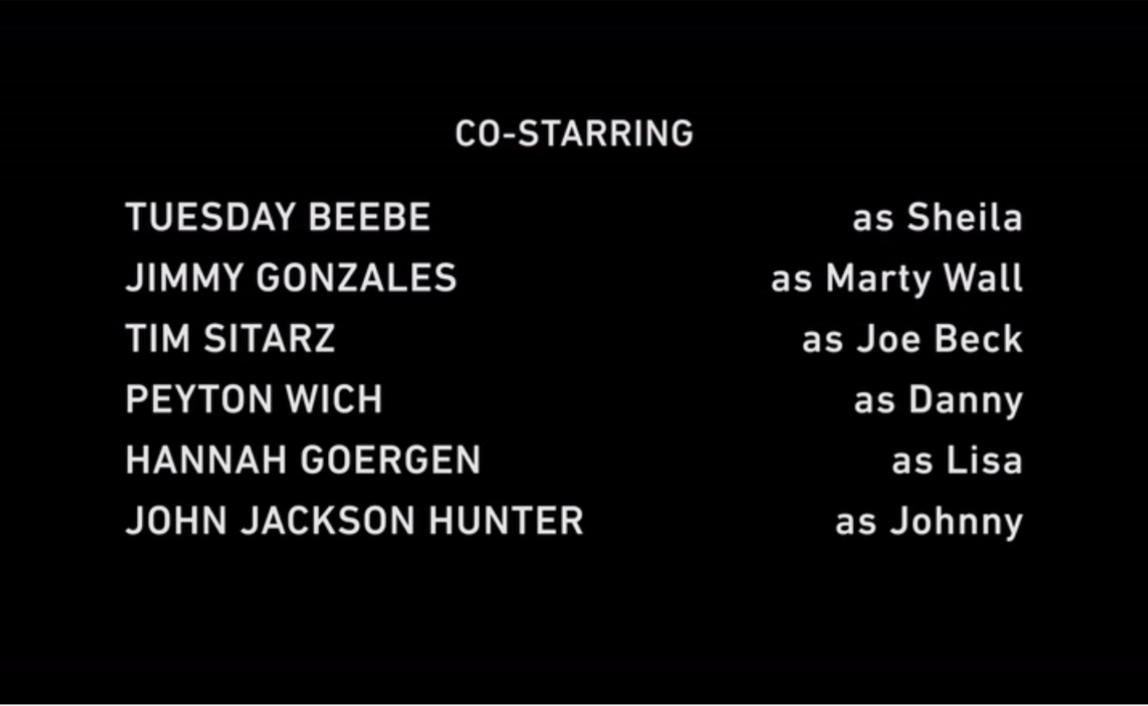
\includegraphics[width=\textwidth]{images/screencreditslarge.png}
  \end{subfigure}
  \begin{subfigure}[b]{0.4\textwidth}
    
\includegraphics[width=\textwidth]{images/screencreditslarge2.png}
  \end{subfigure}
\begin{subfigure}[b]{0.4\textwidth}
	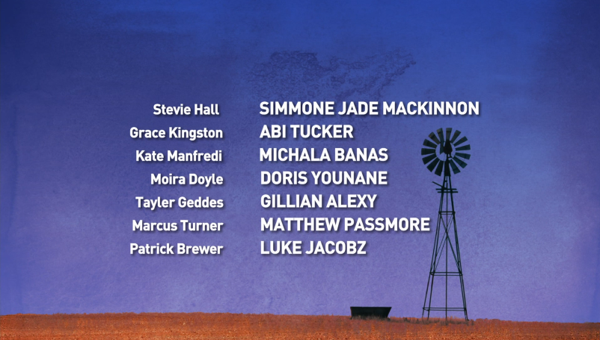
\includegraphics[width=\textwidth]{images/diffcredits.png}
\end{subfigure}
\begin{subfigure}[b]{0.4\textwidth}
	
\includegraphics[width=\textwidth]{images/diffcredits2.png}
\end{subfigure}
  \caption{\textbf{Examples of varying types of closing credits}}
  \label{closingcredits}
\end{figure}

\subsubsection{Opening credits}
The opening credits of a TV-show are generally the same for all of the episodes in the same season. It typically opens the show with a theme song, presenting the most important actors at the start. If the sequence is known beforehand then it would be a rather simple problem to solve, by matching this sequence with all of the videos to locate the opening credits. The difficult part here is that they start somewhere at the start of a video, never right at the start. There is also no prior knowledge on how the opening credits of a show look like and they often change every season.

\subsubsection{Recaps}
A television show typically has recaps before the opening credits. In the recaps content of previous episodes is repeated to refresh the viewer's memory. This is useful for linear TV when an episode is aired every week. Someone watching episodes back-to-back ideally wants to skip the recaps together with the opening credits because they have seen the content recently. Not all material preceding the opening credits is a recap though, sometimes it is original content.

\subsubsection{Bumpers}
The bumper is a part of the video that eases a viewer into the upcoming commercial (see figure \ref{examplebumper}). Most of the times it has a voice over and text on screen saying: 'Next' (or the dutch translation of 'next') and some footage of what is to be expected after the commercial break is shown.

\begin{figure}[H]
    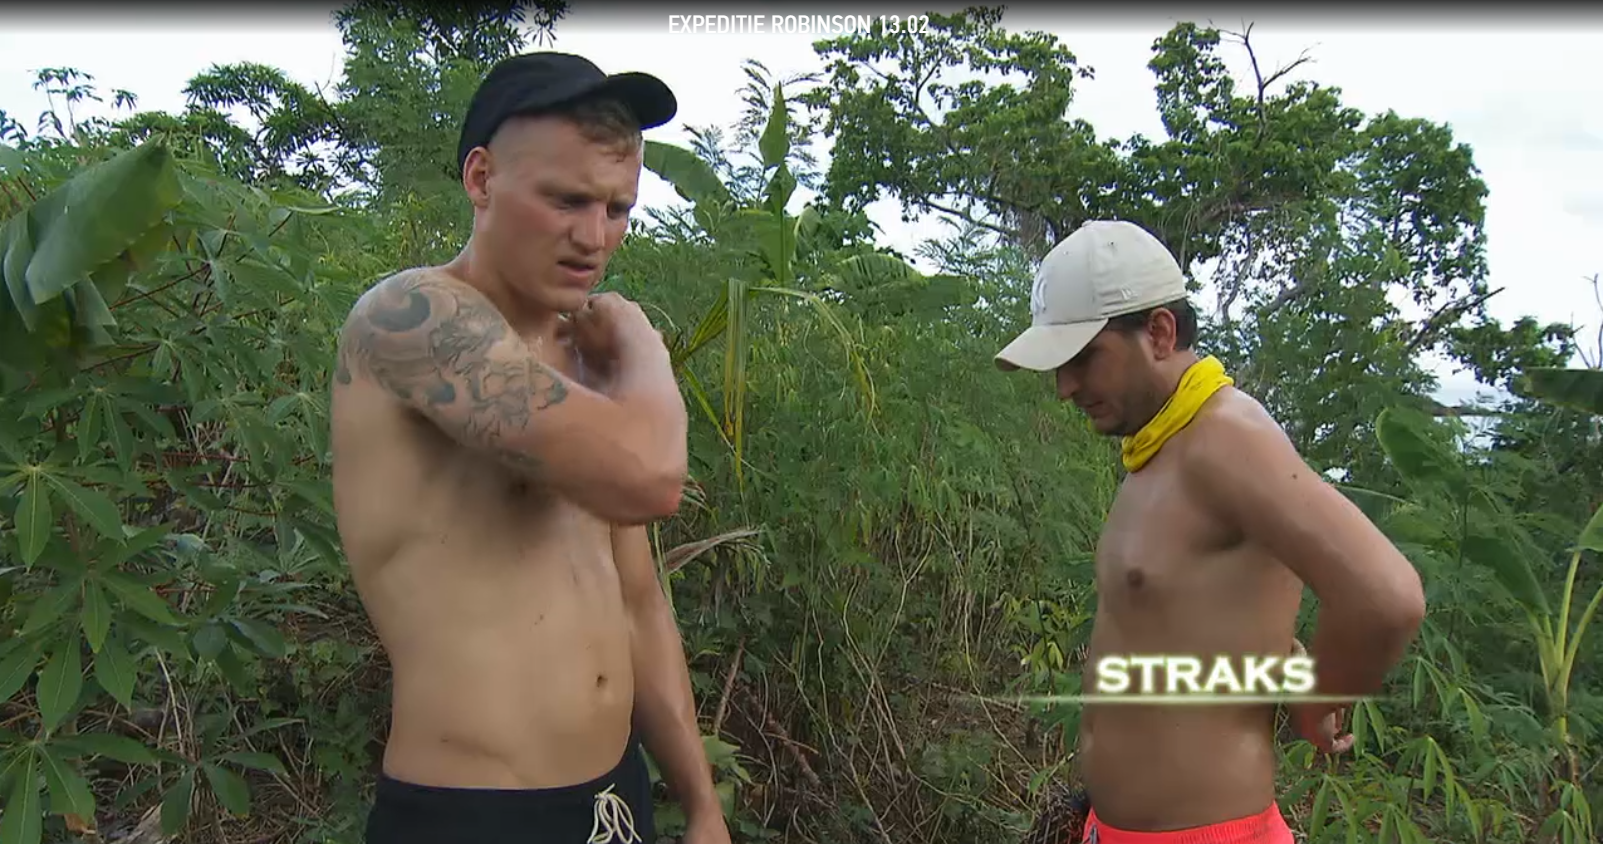
\includegraphics[width=7.5cm]{images/straks.png}
    \centering
    \caption{\textbf{Example 'Next' bumper of the dutch television show Expeditie Robinson.}}
    \label{examplebumper}
\end{figure}

\subsubsection{Previews}
A preview is a segment at the end of an episode where an advance showing of fragments of the next episode(s) are played. Previews can typically be found in content that was created specially for broadcast TV. It gives the viewer a taste of what to expect in the next episode that will air a week later. However, this part is not of interest to someone watching episodes back-to-back.

\subsection{Definitions and Techniques}
This section will be used to elaborate on some topics mentioned in this thesis. We define a season with multiple episodes of a TV-show as T.
\[T = \{E_1, E_2, \dots, E_x\}\]
An episode within a season is defined as a set of frames.
\[E = \{f_1, f_2, \dots, f_y\}\]
The videos contain shot boundaries, we refer the set of locations of shotboundaries as B.
\[B = \{b_1, b_2, \dots, b_z\}\]

\subsubsection{Shot Change Detection}

Shot detection is a technique that can be used on videos to determine shot boundaries, see figure \ref{shotchange} for an example of such a shot change. 

\begin{figure}[H]
	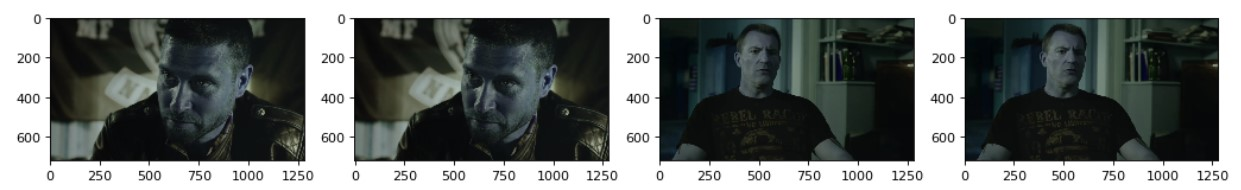
\includegraphics[width=12cm]{images/shotchange.jpg}
	\centering
	\caption{\textbf{Example of a shot change within 4 frames of a video.}}
	\label{shotchange}
\end{figure}

Shot detection is going to be used and thus will we expand on it. A lot of research has been done related to shot detection \cite{lienhart1998comparison} and many techniques have been proposed. 

We use a method that looks at the shift in mean color in HSV space \cite{shao2015shot}. HSV (Hue, Saturation, Value) color space is a more intuitive color mixing model compared to RGB (Red, Green, Blue) color space. Because one can change a value in either of the three values in HSV and expect what the new color is going to look like. This is almost impossible for RGB because for this same color change to happen, you need to change all three red, green and blue values to result in the same color space.

The shot boundaries are classified by calculating the difference in hue, saturation and value for each frame and then from this the mean is calculated. If the mean is higher than a threshold H, then a shot boundary is marked, refer to algorithm \ref{algorithm:shotboundary} for a pseudo-code representation.

\begin{algorithm}[H] 
	\SetAlgoLined
	shotBoundaries = List()\;
	previousMeanHSV = getMeanHSV(Episode[0])\;
	\For{frame in Episode}{
		meanHSV = getMeanHSV(frame)\;
		\If{abs(meanHSV - previousMeanHSV) $>$ H}{
			shotBoundaries.add(frame)\;
		}
		previousMeanHSV = meanHSV\;
	}
	\caption{\textbf{Shot boundary detection}}
	\label{algorithm:shotboundary}
\end{algorithm}

\section{Related Work} \label{relatedwork}

No prior work exists that explores a solution for the problem previously described (automatic labeling of specific repeating segments). Related work exists that focuses on commercial or repeated sequence detection in large broadcast streams. These detection methods can be roughly divided into three groups: fingerprint, feature-based and unsupervised methods. 

%fingerprint
Fingerprint methods set up a database of fingerprints of known commercials or repeated sequences to detect these in a broadcast stream. Lienhart et al.\ \cite{lienhart1997detection} propose a method based on features to roughly localize advertisements in a stream and then construct a fingerprint database based on color coherence vectors. Gauch et al.\ \cite{gauch2006finding} propose a method based on constructing feature vectors from color moments in a stream. Covell et al.\ \cite{covell2006advertisement} implement a fingerprinting method based on audio with visual verification after a proposed match. The disadvantage of these fingerprinting methods is the setting up and maintenance of such a fingerprint database.

%fingerprint methodes geven vaak ook methode voor repeated sequence detection maar met onvoldoende precisie

%feature based
The feature-based methods detect commercials based on extracted video features. Wang et al.\ \cite{wang2008multimodal} fuse the results of audio scene changes and textual content similarity between shots to segment programs including commercials.

%clustering
With the unsupervised methods the authors typically do a dimensionality reduction operation and then try to find repeated sequences or commercials with clustering methods. Herley et al.\ \cite{herley2006argos} convert the stream with a Discrete Cosine Transform (DCT) to reduce dimensionality and then propose an extensive probability framework to detect repeated sequences. Benezeth et al.\ \cite{benezeth2010unsupervised} use the Electronic Programme Guide (EPG) in addition to the dimensionality reduction to detect program boundaries.

%vergelijkbare dingen
Abduraman et al.\ \cite{abduraman2011unsupervised} propose a system to detect repeated sequences in streams by performing a DCT operation on all of the frames in the stream and then use a micro clustering technique to detect repeated sequences. They were also able to link the trailers to their respective programs that occur at a later point in the stream.

All of the previously mentioned works in this section never cover the specific topic of segmenting the classes mentioned in section \ref{section:segmentclasses} or use other properties only available to broadcast streams such as the EPG. The methods yielded high accuracies in the range of 90\% - 95\% precision. This work aims for higher accuracies and thus will not be replicating the previously mentioned methodologies, however from the aforementioned papers we conclude that a large dimensionality reduction step will be necessary to efficiently process a large visual data set.
\\

Dimensionality reduction and efficient matching of large amounts of visual data is important within content based image retrieval, Zheng et al. give a very detailed summary of all the significant contributions from past years \cite{zheng2018sift}. Their summary covers three periods in image retrieval: Early methods, SIFT-based methods and Convolutional Neural Network (CNN) based methods. Smeulders et al. present all the contributions of the early methods \cite{smeulders2000content}, these methods focused on looking at the color, texture and local geometry of images for retrieval \cite{yu2002color,manjunath1996texture}. Not much later the Bag-of-words (BoW) model was proposed as a new method for image retrieval \cite{sivic2003video}. The advantage of this is that inverted indexes can be used for immediate retrieval of similar images. The BoW model paired with SIFT-descriptors \cite{lowe2004distinctive} as the feature vectors was used in image retrieval research for years \cite{nister2006scalable,philbin2007object,jegou2008hamming,jegou2010aggregating,jegou2012aggregating}. Since 2012 when the convolutional neural network was introduced \cite{krizhevsky2012imagenet} research switched to CNN-based methods for image retrieval because they achieved better performance on several image retrieval tasks	 \cite{babenko2014neural,yue2015exploiting, tolias2015particular}.


\iffalse
%oude paper OCR op video
\cite{li2000automatic} %TODO

%fingerprints
\cite{lienhart1997detection} %commercial detection met fingerprints
\cite{covell2006advertisement} %commercial detection fingerprints

%features
\cite{gauch2006finding} %commercial detection features
\cite{wang2008multimodal} %doen programma segmentatie

%clustering
\cite{herley2006argos} %argos paper gebruikt audio en heel veel probability
\cite{berrani2008non} %micro clustering repeated sequence detection

\cite{benezeth2010unsupervised} %enige paper die iets vergelijkbaars doet, maar op basis van stream en programmagids, veel nuttige references
\cite{ibrahim2011tv} %andere vergelijkbare paper, op advertenties en met grote stream
\cite{abduraman2011unsupervised} %Ook hele vergelijkbare paper, werken ook weer met DCT en KVD maar recall en precision round 0.95
\fi


\section{Image Retrieval} \label{section:imageretrieval}
Image retrieval is a subset of the research field Information Retrieval (IR). Explained briefly, it investigates the problem where one has a query \textbf{q} expressing an information need and wants to find the best possible match for this \textbf{q} in a set of documents \textbf{D}.

In the case of image retrieval the query consists of an image for which the best matching image should be found in a document set of images. There are two approaches for doing this.

\begin{figure}[H]
	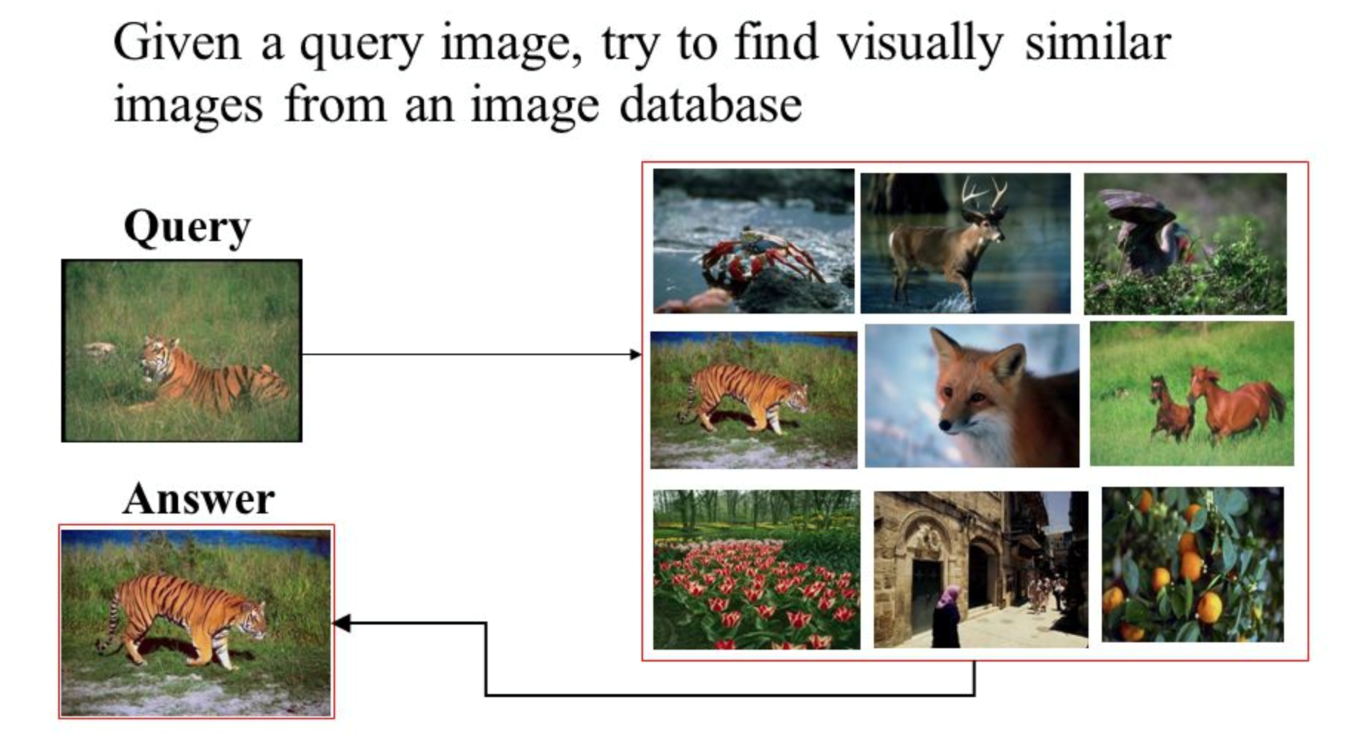
\includegraphics[width=8cm]{images/imageretrieval.png}
	\centering
	\caption{\textbf{Visual example of image retrieval.}}
	\label{fig:imageretrieval}
\end{figure}

\textbf{Text-based image retrieval} refers to retrieval of images based on textual metadata associated with these images. It matches images based on for instance their titles, keywords and more. The downside of this method is that if there is no metadata available then it needs to be added manually. With the growing sizes of image databases this can become quite inefficient, hence the more focus on content-based image retrieval in past years \cite{rajam2013survey}.

\textbf{Content-based image retrieval} is retrieval based on the content of the image rather than the metadata as is the case with concept-based image retrieval. Computer vision is used to evaluate the image similarity, this can be done by looking at colors, shapes, textures and more. The advantage of content based image retrieval is that it does not rely on the metadata of images and thus does not require manual labeling.

\subsection{Feature vectors}
%TODO: veranderen in kleurencounts wit en zwart
A feature vector is a vector containing a numeric representation of multiple characteristics of an object. In this case the objects will be images, the frames of a video. To illustrate feature vectors for images, a small example will be given. Consider the following three images of 10 by 10 pixels consisting only of black or white pixels. 

\begin{figure}[H]
	\centering
	\begin{subfigure}[b]{0.2\textwidth}
		
\includegraphics[width=\textwidth]{images/mostlywhite.png}
	\end{subfigure}
	\begin{subfigure}[b]{0.2\textwidth}
		
\includegraphics[width=\textwidth]{images/allblack.png}
	\end{subfigure}
	\begin{subfigure}[b]{0.2\textwidth}
		
\includegraphics[width=\textwidth]{images/mostlyblack.png}
	\end{subfigure}
	\caption{\textbf{Three images of 10x10 pixels, consisting of only black and white pixels. The resulting feature vectors are $[64,36]^T$, $[0, 100]^T$ and $[25,75]^T$ respectively.}}
	\label{featurevectorimages}
\end{figure}

If we would like to measure the image similarity between these pictures then we could do this on a pixel-per-pixel basis, this could work for low dimensional images. But comparing HD images consisting of 1920 pixels by 1080 pixels would require massive computation and will not be able to handle small deviations between images. This can be resolved by creating feature vectors to represent the images. A representation for these example images could be the number of black and white pixels in the image. This results in the feature vector $\textbf{x} = [\# white pixels, \# black pixels]^T$. This vector can now be represented in 2D-space, and compared to other vectors in 2D space by calculating the distance between other points in that space. The distance is computed by calculating the euclidean distance between each vector.

\[d(\textbf{p,q}) = \sqrt{(p_1 - q_1)^2 + \dots + (p_n - q_n)^2} \]

In figure \ref{fig:distanceexample} the plotted feature vectors and the distances between them can be viewed. Example images 2 and 3 are the most alike because the distance between them is the smallest. 

\begin{figure}[H]
	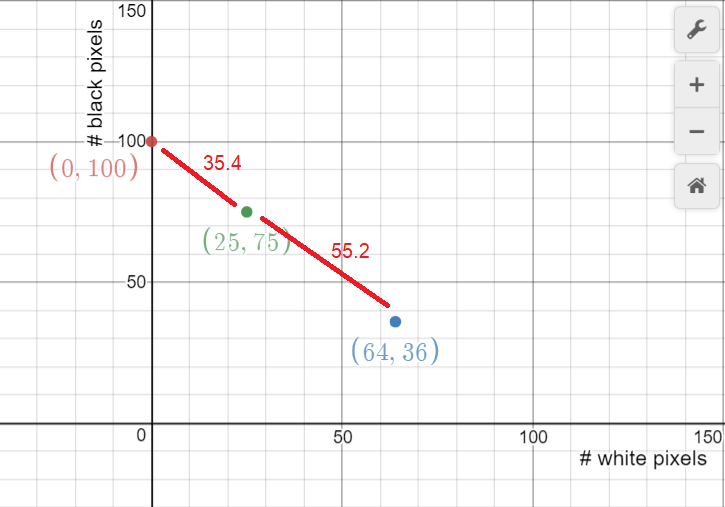
\includegraphics[width=8cm]{images/distanceexample.png}
	\centering
	\caption{\textbf{Example of distance in 2D between feature vectors that represent the example images. According to the chosen features, image 2 and 3 are the most alike.}}
	\label{fig:distanceexample}
\end{figure}

The similarity of images can be retrieved by computing the distance between their feature vectors. A low distance indicates a higher similarity. Counting the number of black and white pixels for the construction of feature vectors is not a very robust method. Many research in image retrieval has been done on the construction of these feature vectors for achieving the best retrieval results. Part of this research is determining the best method for the construction of the image feature vectors to apply for our problem. We will expand on the methods that are going to be explored. 

%Misschien uitwijden over local en global descriptors
As mentioned in section \ref{relatedwork}, Zheng et al. \cite{zheng2018sift} outline three significant periods in image retrieval, the early methods focused on global descriptors based on color and texture. These global descriptors were not good at handling image changes in illumination, translation, occlusion and truncation. This gave rise to local descriptors based SIFT methods until recently CNN-descriptors became the most popular. 

Initially the plan was to experiment with a method out of each of these three periods. However, early experimentation indicated that SIFT methods would be too inefficient for our application. That is why we settled on trying out color histograms as a global descriptor, local color texture moments \cite{yu2002colortexturemoments} as a method that tries to describe the image on a less global level by taking texture of the image into account. Finally CNN-descriptors as local descriptors.

This is not an exhaustive list of methods, but because computing feature vectors for a large amount of frames is resource intensive, we limited ourselves to these three. If one of the methods achieves promising results then future research can expand on variations of the method or if none of the methods achieve acceptable results, then future research could try other distinct methods.

\subsection{Color Histograms}
A color histogram is a representation of the distribution of colors in an image. Color histograms are a flexible and low dimensional way of representing images. A color histogram can be computed by counting the number of pixels in a certain color range, the size of this range is variable, called the bin size. A larger bin size results in lower dimensions of the resulting histogram. For example, if one chooses a bin size that is half of the intensity range. The resulting vector would have 6 dimensions, two bins for each color channel. See figure \ref{fig:colorhistogram} for an example with such a bin size.
\begin{figure}[H]
	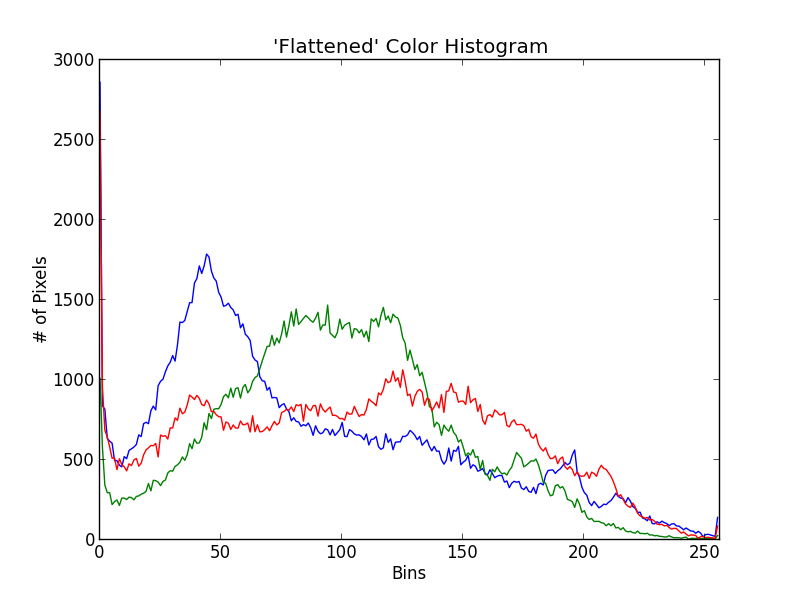
\includegraphics[width=8cm]{images/colorhistogram.png}
	\centering
	\caption{\textbf{Color histogram with a large binsize (binsize=128) for illustration.}}
	\label{fig:colorhistogram}
\end{figure}
Color histograms are global descriptors because they describe the image on a global level.

\subsection{Color Texture Moments}
Color texture moments as proposed by Yu et al. \cite{yu2002colortexturemoments} are a low-level feature descriptor that integrates both color and texture characteristics of an image. An image is converted from RGB to HSV color space, and on each color map a 2d convolution is applied for each filter shown in figure \ref{fig:filters}.

\begin{figure}[H]
	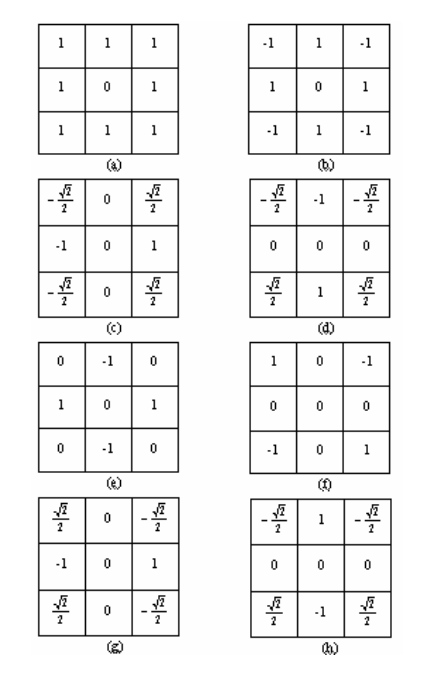
\includegraphics[width=5cm]{images/filters.png}
	\centering
	\caption{\textbf{Filters used for computing the color texture channels.}}
	\label{fig:filters}
\end{figure}

Which results in 8 channels for each color map, 24 channels in total. For each of the resulting channels the first and second color moments, which are the mean and standard deviation, are taken. This results in a 48-dimensional feature vector.

\subsection{CNN Features} 
Convolutional neural networks are very good at image classification and segmentation tasks. However it was found that using the resulting channels after the convolution layers as feature vectors also perform well at image retrieval tasks.
TODO EXPAND

\section{Methodology} \label{methodology}
We want to explore whether we can detect recurring content unsupervised and if so, which method scores the best in terms of accuracy and efficiency. Initially a non-generalized approach was started with, where a unique method for each content class was tried (For example: OCR for textual closing credits and similarity matrices for opening credits). This was found to be ineffective because of a high variety of edge cases. 

The characteristic of all the segment classes is that they reoccur either in previous or future episodes. To match frames from one episode with other episodes, feature vectors will be constructed from the frames and the distances between these vectors will be computed and saved. If a part of the video consecutively has matching feature vectors from previous or future episodes, then that part is labeled as a recurring segment. It is therefore important that the resulting feature vectors do not mismatch between actual recurring content and content that looks alike. Methods chosen for construction of the feature vectors should therefore not result in feature vectors of very high dimensionality, because this has proven to reduce the distance between the farthest and closest points \cite{beyer1999nearest}, diminishing the distinctive property of the feature vectors that is needed. 

\subsection{Data}
The data set contains 83 video files originating from 16 different seasons of tv-shows, amounting to around 50 hours of content. Of most seasons only the first few episodes will be looked at to have a more varied data set. Originally these files were in .mxf full broadcast format, this meant each file being 25GB on average. All the files were converted to 1920p .mp4 files with FFmpeg \cite{ffmpeg}, resulting in each file being around 1 GB on average.

For each file the start and end timestamps for the recaps, opening credits, closing credits and previews were annotated in the HH:MM:SS format in a CSV file, so that it could be loaded and compared effectively.

\subsection{Feature Vector Construction}
Video generally plays at 25 frames per second, frames very close to each other should only have very slight variations. That is why frames every 5 frames or just shotboundary frames will be taken into account to drastically reduce the computing complexity. We take all the video files of a season $E_x \in T$ and convert each file to a set of feature vectors $S_x = \{v_1, v_2, \dots, v_l\}$ with the function $f$.

\[f(E_x) = S_x = \{v_1, v_2, \dots, v_l\}\]

The rest of the subsections will expand on different implementations of the function $f$, how the different types of feature vectors are constructed. We use three different methods for the feature vector construction. These methods were chosen because of their efficient computation and accuracy in image retrieval tasks. The methods chosen were color histograms, local color texture moments and CNN features.

\subsubsection{Color Histograms}
For the construction of the color histograms the pixels intensities in each channel (Red, Green, Blue (RGB)) are counted and binned according to a specified bin size. All these bins will be concatenated to result in a feature vector, the size of the feature vector is a result of the chosen bin size.

We use 30 bins to represent a single color channel. These are then concatenated into a 1D vector, resulting in a feature vector with a dimensionality of 90. The values are normalized by dividing each bin with the sum of all bins.

\[H = \frac{H_x}{\sum H_i} \]

A histogram is computed for every 5 frames in the video and then stored and saved in a list that preserves the order.

\subsubsection{Local Color Texture Moments}
TODO

\subsubsection{CNN Features}
TODO

\subsection{Matching and Detection}

All the resulting lists of feature vectors will be added to the index of an empty Faiss instance. Faiss is a library for efficient similarity search of dense vectors \cite{faiss, faiss-github} and thus perfectly suited for our task. This library will efficiently handle building the inverted index and nearest neighbor matching. The science that is behind large scale matching of dense vectors is a research field in itself, but outside the scope of this thesis. We use Faiss because it is released as an open source library and therefore easy to use in an implementation.

\begin{figure}[H]
	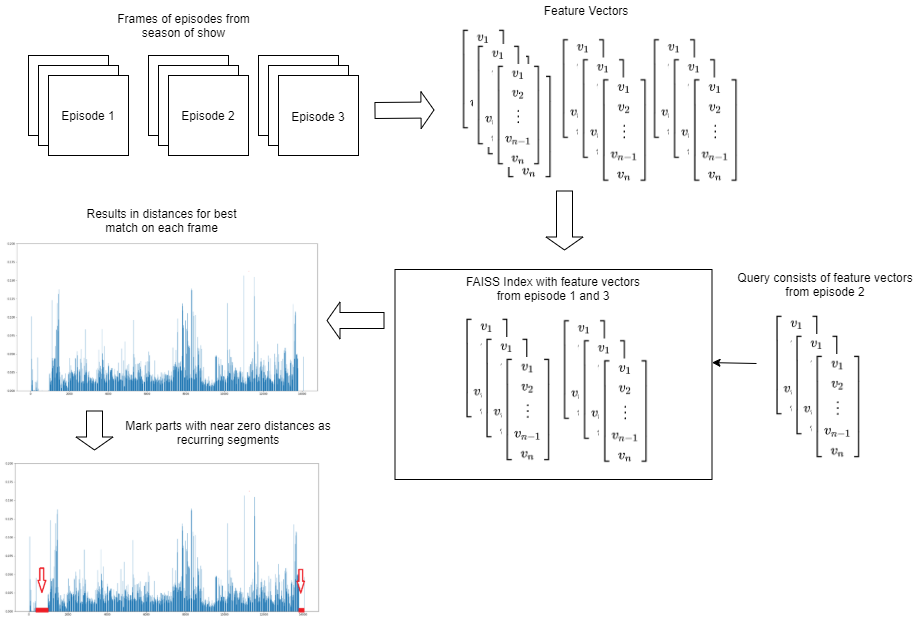
\includegraphics[width=\paperwidth, center, scale=0.7]{images/thesisdiagram.png}
	\centering
	\caption{\textbf{Diagram of the described methodology. The recurrent content detection process for episode 2 is portrayed.}}
	\label{fig:diagram}
\end{figure}

All distances up until the 5th percentile will be taken into consideration. This is because on average 3.7\% of the content was skippable on average for the data that was used.

\subsubsection{Bumper Detection}
The methodology for detecting the bumpers within video content is different. Because a bumper only contains recurring content from within the video itself. It shows shots that will be shown after the break, these shots may not reoccur in other episodes within a season. Therefore we cannot use the same methodology as described before for detection.

For the detection of bumpers we take a sliding window of 18 seconds of video frames, this will be the query. The index will consist of the remaining frames in the video, the resulting distances of the two nearest neighbors will be saved and then this process is repeated for the next 18 seconds in the video.

After all the closest in-episode nearest neigbors are computed for each frame then from these results bumpers can be detected. We found that a global threshold for determining matches does not work well, probably because of the fact that bumpers are very short. Therefore we will use the ratio test described by Lowe \cite{lowe2004distinctive} for deciding on whether there is a match. With the ratio test the distance between the closest neighbor and second-closest neighbor is taken into account. The ratio of the distance of the closest neighbor to the distance of the second-closest neighbor determines whether there is a correct match, if the ratio is low then there is a higher chance for the match to be correct. In \cite{lowe2004distinctive} they classify a match to be correct if the ratio of the distances is equal to 0.8 or lower, we will however use a ratio of 0.7, to slightly reduce the number of false positive matches.



\section{Results} \label{results}

The results will be evaluated as a retrieval problem. By doing so, the measures precision and recall could be used to describe several aspects of each method. Each second of recurrent content is marked as a relevant instance and if recurrent content gets detected, then those are relevant detected seconds, by doing so we can calculate precision and recall as following:

\[\mathrm{precision} = \frac{\mathrm{detected\;relevant\;seconds}}{\mathrm{detected\;seconds}}\]

\[\mathrm{recall} = \frac{\mathrm{detected\;relevant\;seconds}}{\mathrm{total\;relevant\;seconds}}\]

\[F1 = \frac{2*\mathrm{recall} * \mathrm{precision}}{\mathrm{recall} + \mathrm{precision}}\]

Because it is possible for the annotation to be slightly inaccurate, we mark detections that are within a 2 second margin of the relevant section, to also be relevant.

\begin{center}
	\begin{tabular}{ |c||c|c|c| } 
		\hline
		\textbf{Method} & \textbf{Precision} & \textbf{Recall} & \textbf{F1} \\
		\hline
		CH & cell5 	& cell6 & \\ 
		CTM & cell8 & cell9 & \\ 
		CNN & 		& 		& \\		
		\hline
	\end{tabular}
\end{center}

\subsection{Bumper detection}
Because bumpers are short segments, the bumpers were evaluated in a slight different manner. We will not calculate precision and recall based on numbers of retrieved relevant seconds but whether a detection has overlap with a bumper. If a detection has overlap with a bumper, then this detection is marked as relevant. Precision and recall will thus be calculated according to the following formulas:

\[\mathrm{precision} = \frac{\mathrm{detections\;with\;overlap}}{\mathrm{total\;detections}}\]

\[\mathrm{recall} = \frac{\mathrm{detections\;with\;overlap}}{\mathrm{total\;bumpers\;in\;episode}}\]

The F1 score will be calculated according to the same formula as described before.

\begin{center}
	\begin{tabular}{ |c||c|c|c| } 
		\hline
		\textbf{Method} & \textbf{Precision} & \textbf{Recall} & \textbf{F1} \\
		\hline
		CH & cell5 	& cell6 & \\ 
		CTM & cell8 & cell9 & \\ 
		CNN & 		& 		& \\		
		\hline
	\end{tabular}
\end{center}

\section{Discussion} \label{discussion}

- I did not do an extensive study on all of the TV shows, so other edge cases are possible in other TV-shows.\\
- Very similar scenes occur regardless if it is a skippable segment or not\\
- Distances can be hard to navigate\\
- Using full seasons might give different results
- Video content is creative, never a clear structure, can encounter weird things (Changing of opening credit scenes, dismissal of opening credit scenes, rebroadcast of same content without it being a recap)
- Flash forwards/backwards confuse the model

Answer the following subquestions:
\\
\textit{\textbf{How can image retrieval be used to detect recurring content?\newline}}\\
\textit{\textbf{How accurate is each image retrieval approach?\newline}}\\
\textit{\textbf{How can the best method be utilized in practice?\newline}}

Then the main question:
\textit{\textbf{How well do image retrieval methods perform in accurately detecting recurring content across a TV-show?\newline}}

Then draw a conclusion

\bibliographystyle{ieeetr}
\bibliography{references}

\end{document}
